\documentclass{article}

\usepackage{amsmath,amssymb}
\usepackage{tikz}
\usepackage{pgfplots}
\usepackage{xcolor}
\usepackage[left=2.1cm,right=3.1cm,bottom=3cm,footskip=0.75cm,headsep=0.5cm]{geometry}
\usepackage{enumerate}
\usepackage{enumitem}
\usepackage{marvosym}
\usepackage{tabularx}
\usepackage[amsmath,thmmarks,standard]{ntheorem}
\usepackage{mathtools}

\usepackage[utf8]{inputenc}

\renewcommand*{\arraystretch}{1.4}
\newcommand{\E}{\mathbb{E}}

\newcolumntype{L}[1]{>{\raggedright\arraybackslash}p{#1}}
\newcolumntype{R}[1]{>{\raggedleft\arraybackslash}p{#1}}
\newcolumntype{C}[1]{>{\centering\let\newline\\\arraybackslash\hspace{0pt}}m{#1}}

\DeclareMathOperator{\tr}{tr}
\DeclareMathOperator{\Var}{Var}
\DeclareMathOperator{\Cov}{Cov}
\renewcommand{\E}{\mathbb{E}}

\newtheorem{thm}{Theorem}
\newtheorem{lem}{Lemma}

\title{\textbf{Einführung in die Logistik, Übung 2}}
\author{\textsc{Henry Haustein}}
\date{}

\begin{document}
	\maketitle
	
	\section*{Aufgabe 3}
	\begin{enumerate}[label=(\alph*)]
		\item[(b)] Man sieht recht schnell, dass die Knoten 1,2 und 5 mit 2 Kanten verbunden sind und dass die Knoten 4 und 6 mit einer Kante verbunden sind. Wir haben also 2 Bäume, da jeweils $\vert V\vert = \vert E\vert - 1$ gilt.
		\item[(c)] Die Adjazenzmatrix lautet
		\begin{align}
			A(Z(\vec{G}))=\begin{pmatrix}
				0 & 1 & 0 & 0 & 1 & 0 \\
				1 & 0 & 0 & 0 & 1 & 0 \\
				0 & 0 & 0 & 1 & 0 & 1 \\
				0 & 0 & 1 & 0 & 0 & 1 \\
				1 & 1 & 0 & 0 & 0 & 0 \\
				0 & 0 & 1 & 1 & 0 & 0
			\end{pmatrix} \notag
		\end{align}
		\item[(d)] Graph
		\begin{center}
			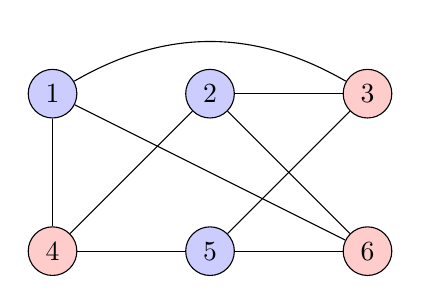
\begin{tikzpicture}
			\node[circle,draw=black, fill=blue!20] (1) at (0,0) {1};
			\node[circle,draw=black, fill=blue!20] (2) at (2,0) {2};
			\node[circle,draw=black, fill=red!20] (3) at (4,0) {3};
			\node[circle,draw=black, fill=red!20] (4) at (0,-2) {4};
			\node[circle,draw=black, fill=blue!20] (5) at (2,-2) {5};
			\node[circle,draw=black, fill=red!20] (6) at (4,-2) {6};
			
			\draw (1) to[bend left=30] (3);
			\draw (1) -- (4);
			\draw (1) -- (6);
			\draw (2) -- (3);
			\draw (2) -- (4);
			\draw (2) -- (6);
			\draw (3) -- (5);
			\draw (4) -- (5);
			\draw (5) -- (6);
			\end{tikzpicture}
		\end{center}
		\item[(e)] ist bei Anblick des Graphen ziemlich offensichtlich
	\end{enumerate}

	\section*{Aufgabe 4}
	\begin{enumerate}[label=(\alph*)]
		\item $G$ ist genau dann topologisch sortiert genau dann wenn für jeden Pfeil von $i$ nach $j$ gilt: $i<j$.
		\item $G$ muss zyklenfrei sein.
		\item  z.B. dieser Graph ist topologisch sortiert:
		\begin{center}
			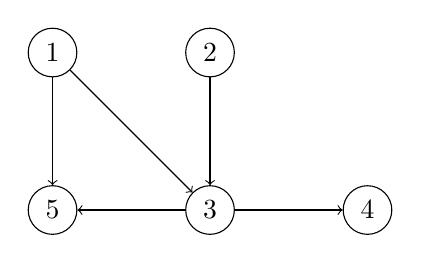
\begin{tikzpicture}
			\node[circle,draw=black, fill=white] (1) at (0,0) {1};
			\node[circle,draw=black, fill=white] (2) at (2,0) {2};
			\node[circle,draw=black, fill=white] (3) at (2,-2) {3};
			\node[circle,draw=black, fill=white] (4) at (4,-2) {4};
			\node[circle,draw=black, fill=white] (5) at (0,-2) {5};
			
			\draw[->] (1) -- (5);
			\draw[->] (1) -- (3);
			\draw[->] (2) -- (3);
			\draw[->] (3) -- (5);
			\draw[->] (3) -- (4);
			\end{tikzpicture}
		\end{center}
	\end{enumerate}
	
	\section*{Aufgabe 5}
	\begin{enumerate}[label=(\alph*)]
		\item Ich fande die Erklärung des Algorithmus in der Vorlesung ziemlich schlecht, deswegen hier noch mal die Kurzfassung:
		\begin{enumerate}[label=\arabic*.]
			\item Sortieren aller Gewichte
			\item Diese Liste vom kleinsten zum größten Gewicht abarbeiten, indem man die Knoten, zu denen das die Kante mit dem Gewicht gehört, ins Gerüst aufnehmen.
			\item Ein Gewicht darf nicht verwendet werden, wenn mit den bereits im Gerüst vorhandenen Kanten durch die neue Kante ein Zyklus entstehen würde.
		\end{enumerate}
		Dieses Verfahren liefert das folgende Minimalgerüst
		\begin{center}
			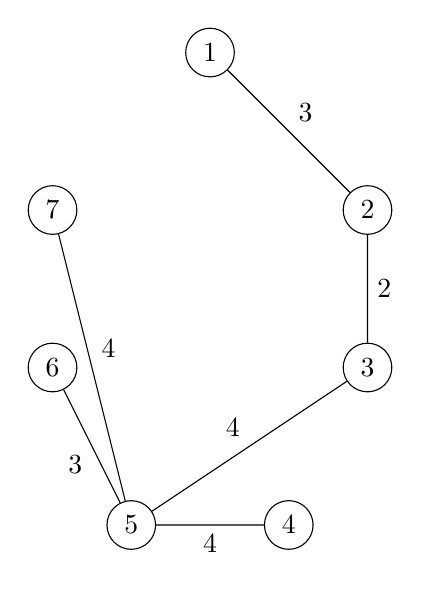
\begin{tikzpicture}
			\node[circle,draw=black, fill=white] (1) at (0,0) {1};
			\node[circle,draw=black, fill=white] (2) at (2,-2) {2};
			\node[circle,draw=black, fill=white] (3) at (2,-4) {3};
			\node[circle,draw=black, fill=white] (4) at (1,-6) {4};
			\node[circle,draw=black, fill=white] (5) at (-1,-6) {5};
			\node[circle,draw=black, fill=white] (6) at (-2,-4) {6};
			\node[circle,draw=black, fill=white] (7) at (-2,-2) {7};
			
			\draw (1) to node[above right] {3} (2) to node[right] {2} (3) to node[above left] {4} (5) to node[below left] {3} (6);
			\draw (4) to node[below] {4} (5) to node[above right] {4} (7);
			\end{tikzpicture}
		\end{center}
		\item Es gibt eine sehr schöne Schreibweise für den Ablauf des Algorithmus aus der Vorlesung \textit{Einführung in die Informatik}. Dabei ist die Menge $S$ die Menge der bisher erkundeten Punkte, zu diesen Punkten kennt man den kürzesten Weg und $D(i)$ ist die (kumulierte) Distanz zum Knoten $i$.
		\begin{center}
			\begin{tabular}{c|c|cccccc}
				Iteration & $S$ & $D(1)$ & $D(2)$ & $D(4)$ & $D(5)$ & $D(6)$ & $D(7)$ \\
				\hline
				0 & $\{3\}$ & 7 & $\infty$ & $\infty$ & $\infty$ & $\infty$ & $\infty$ \\
				1 & $\{1,3\}$ & 7 & 10 & $\infty$ & $\infty$ & $\infty$ & 12 \\
				2 & $\{1,2,3\}$ & 7 & 10 & $\infty$ & 19 & $\infty$ & 12 \\
				3 & $\{1,2,3,7\}$ & 7 & 10 & $\infty$ & 16 & $\infty$ & 12 \\
				4 & $\{1,2,3,5,7\}$ & 7 & 10 & 21 & 16 & $\infty$ & 12 \\
				5 & $\{1,2,3,4,5,7\}$ & 7 & 10 & 21 & 16 & 27 & 12 \\
				6 & $\{1,2,3,4,5,6,7\}$ & 7 & 10 & 21 & 16 & 27 & 12
			\end{tabular}
		\end{center}
	\end{enumerate}
	
\end{document}